% !TEX root = ../notes_template.tex
\chapter{Respiration}\label{chp:blood_oxygen}
Updated on \today
\minitoc
This chapter covers blood support of the extracellular fluid and cellular function by having the correct blood gases which is supported through Pulmonary (external) Respiration. Respiration is a microcirculation process that therefore requires concentration and pressure gradients as well as blood transport and circulation. Cellular (internal) Respiration occurs between the capillaries and muscle fibers and is supported by circulation. Pulmonary (external) Respiration is supported by Pulmonary Circulation (covered in this chapter). Just as Cellular Respiration includes a micro-circulatory exchange with muscle fibers, Pulmonary Respiration includes a micro-circulatory exchange with the the alveoli (air sacs) in the lung. Alveolar ventilation (covered in the next chapter) ensures that the alveoli maintain the required concentration (pressure) of both $CO_2$ and $O_2$ to support Pulmonary Respiration.

\vspace{5mm}

\textbf{Objectives include:}
\begin{enumerate}
    \item
    \item
    \item
    \item
    \item
\end{enumerate}

\section{Respiration Overview}
Muscle function requires energy in the form of ATP. Sustained regeneration of ATP in the mitochondria continuously produces $CO_2$ that must be removed from the muscle fiber, and requires $O_2$ which must be delivered to the muscle fiber. The microcirculation removes and provides what the muscle fibers need, including the removal of $CO_2$ and delivery of $O_2$ (Cellular Respiration). The microcirculation of the blood gases from and into muscle fibers requires a concentration gradient that requires a continuous circulation of blood to the muscle capillary network. Blood provides a transport mechanism for both $CO_2$ and $O_2$ (Blood Transport). The circulation of blood from the muscles through veins to the right side of the heart delivers all blood (venous return) to the pulmonary circulation. The pulmonary circulation delivers venous blood through pulmonary arteries to the interstitial space surrounding alveoli (air sacs) in the lungs (Pulmonary Circulation). Microcirculation (primarily gas diffusion) results in the equilibration of blood gases with the alveoli gases (Pulmonary Respiration). Pulmonary circulation then returns arterial blood through pulmonary veins to the left side of the heart for system wide distribution.


\section{Cellular Respiration}

The beginning of cellular respiration occurs inside the mitochondria with aerobic metabolism. It is aerobic metabolism that utilizes $O_2$ and produces $CO_2$ in sufficient quantities to require continuous exchange with the sarcoplasm, interstitial space, circulating blood and ultimately the environment (gas exchange). Cellular respiration establishes the need for what can be referred to as internal respiration, the gas exchange of $O_2$ and $CO_2$ between the intracellular and extracellular (both interstitial and vascular compartments. For simplicity we will use the terms cellular and internal respiration interchangeably.

\subsection{Partial Pressure Gradients \& Diffusion}

The fundamental concept for respiration is that partial pressure gradients of $O_2$ and $CO_2$ create pressure driven flow. For gases, pressure driven flow is typically called diffusion. There is a relationship between concentration and partial pressure. The higher the concentration of a particular molecule in a gas (as a fraction of all the molecules), the higher the partial pressure. Specifically, the partial pressure of a particular molecule in a gas is proportional to the number of particular molecules as a fraction of the total molecules of the gas multiplied by the total pressure of the gas. The partial pressure of $O_2$ being:

\begin{equation}
    PO_2 = FO_2 \times Total Pressure (mmHg)
    \label{PO2}
\end{equation}

Where $FO_2$ is the fraction of $O_2$ in the gas resulting in total pressure ($mmHg$). Air in the environment tends to have 21\% oxygen (as a fraction, 0.21). Air in the environment is inspired so is the fraction of inspired oxygen ($F_iO_2$). At sea level the total air pressure is 760 $mmHg$ (barometric pressure). Therefore, the $F_iO_2 = 0.21 \times 760 mmHg$, so $F_iO_2 = 159.5 mmHg$. 

\subsection{Partial Pressure Driven Diffusion}

Figure \ref{fig:ecf_respiration} is from Chapter \ref{chp:ecf_microcirculation}. Note that the gradients for $O_2$ and $CO_2$ are depicted as partial pressures ($PO_2$ and $PCO_2$). The partial pressure of each compartment is further noted with a subscript, with partial pressure of oxygen in the cell being $P_cO_2$ and in the tissue as $P_tO_2$. The gradient for $PO_2$ is from the arterial end of the capillary (partial pressure of arterial blood, $P_aO_2 \approx 100 mmHg$) into the tissue ($P_tO_2 \approx 40 mmHg$), and into the cell ($P_cO_2 \approx 20 mmHg$). Of these values the $P_cO_2$ is most variable and depends on the rate of utilization of $O_2$ in the mitochrondria (ETC). The partial pressure driven diffusion of cellular respiration relies on the continuous use of $O_2$ in the mitochondria; and the continuous use of $O_2$ in the mitochondria depends on the availability of $O_2$ diffusing in from the arterial blood in the capillary. If aerobic metabolism in a cell stopped then the $P_cO_2$ would quickly equilibrate with the $P_aO_2$ at 100 $mmHg$. If blood flow stopped (ischemia), or if there was a lower partial pressure of oxygen in the arterial blood ($P_aO_2 \leq 60 mmHg$) (hypoxemia) then diffusion of $O_2$ would be slower and the rate of aerobic metabolism (ETC in particular) would be limited (hypoxia).

\begin{figure}[!h]
    \centering
    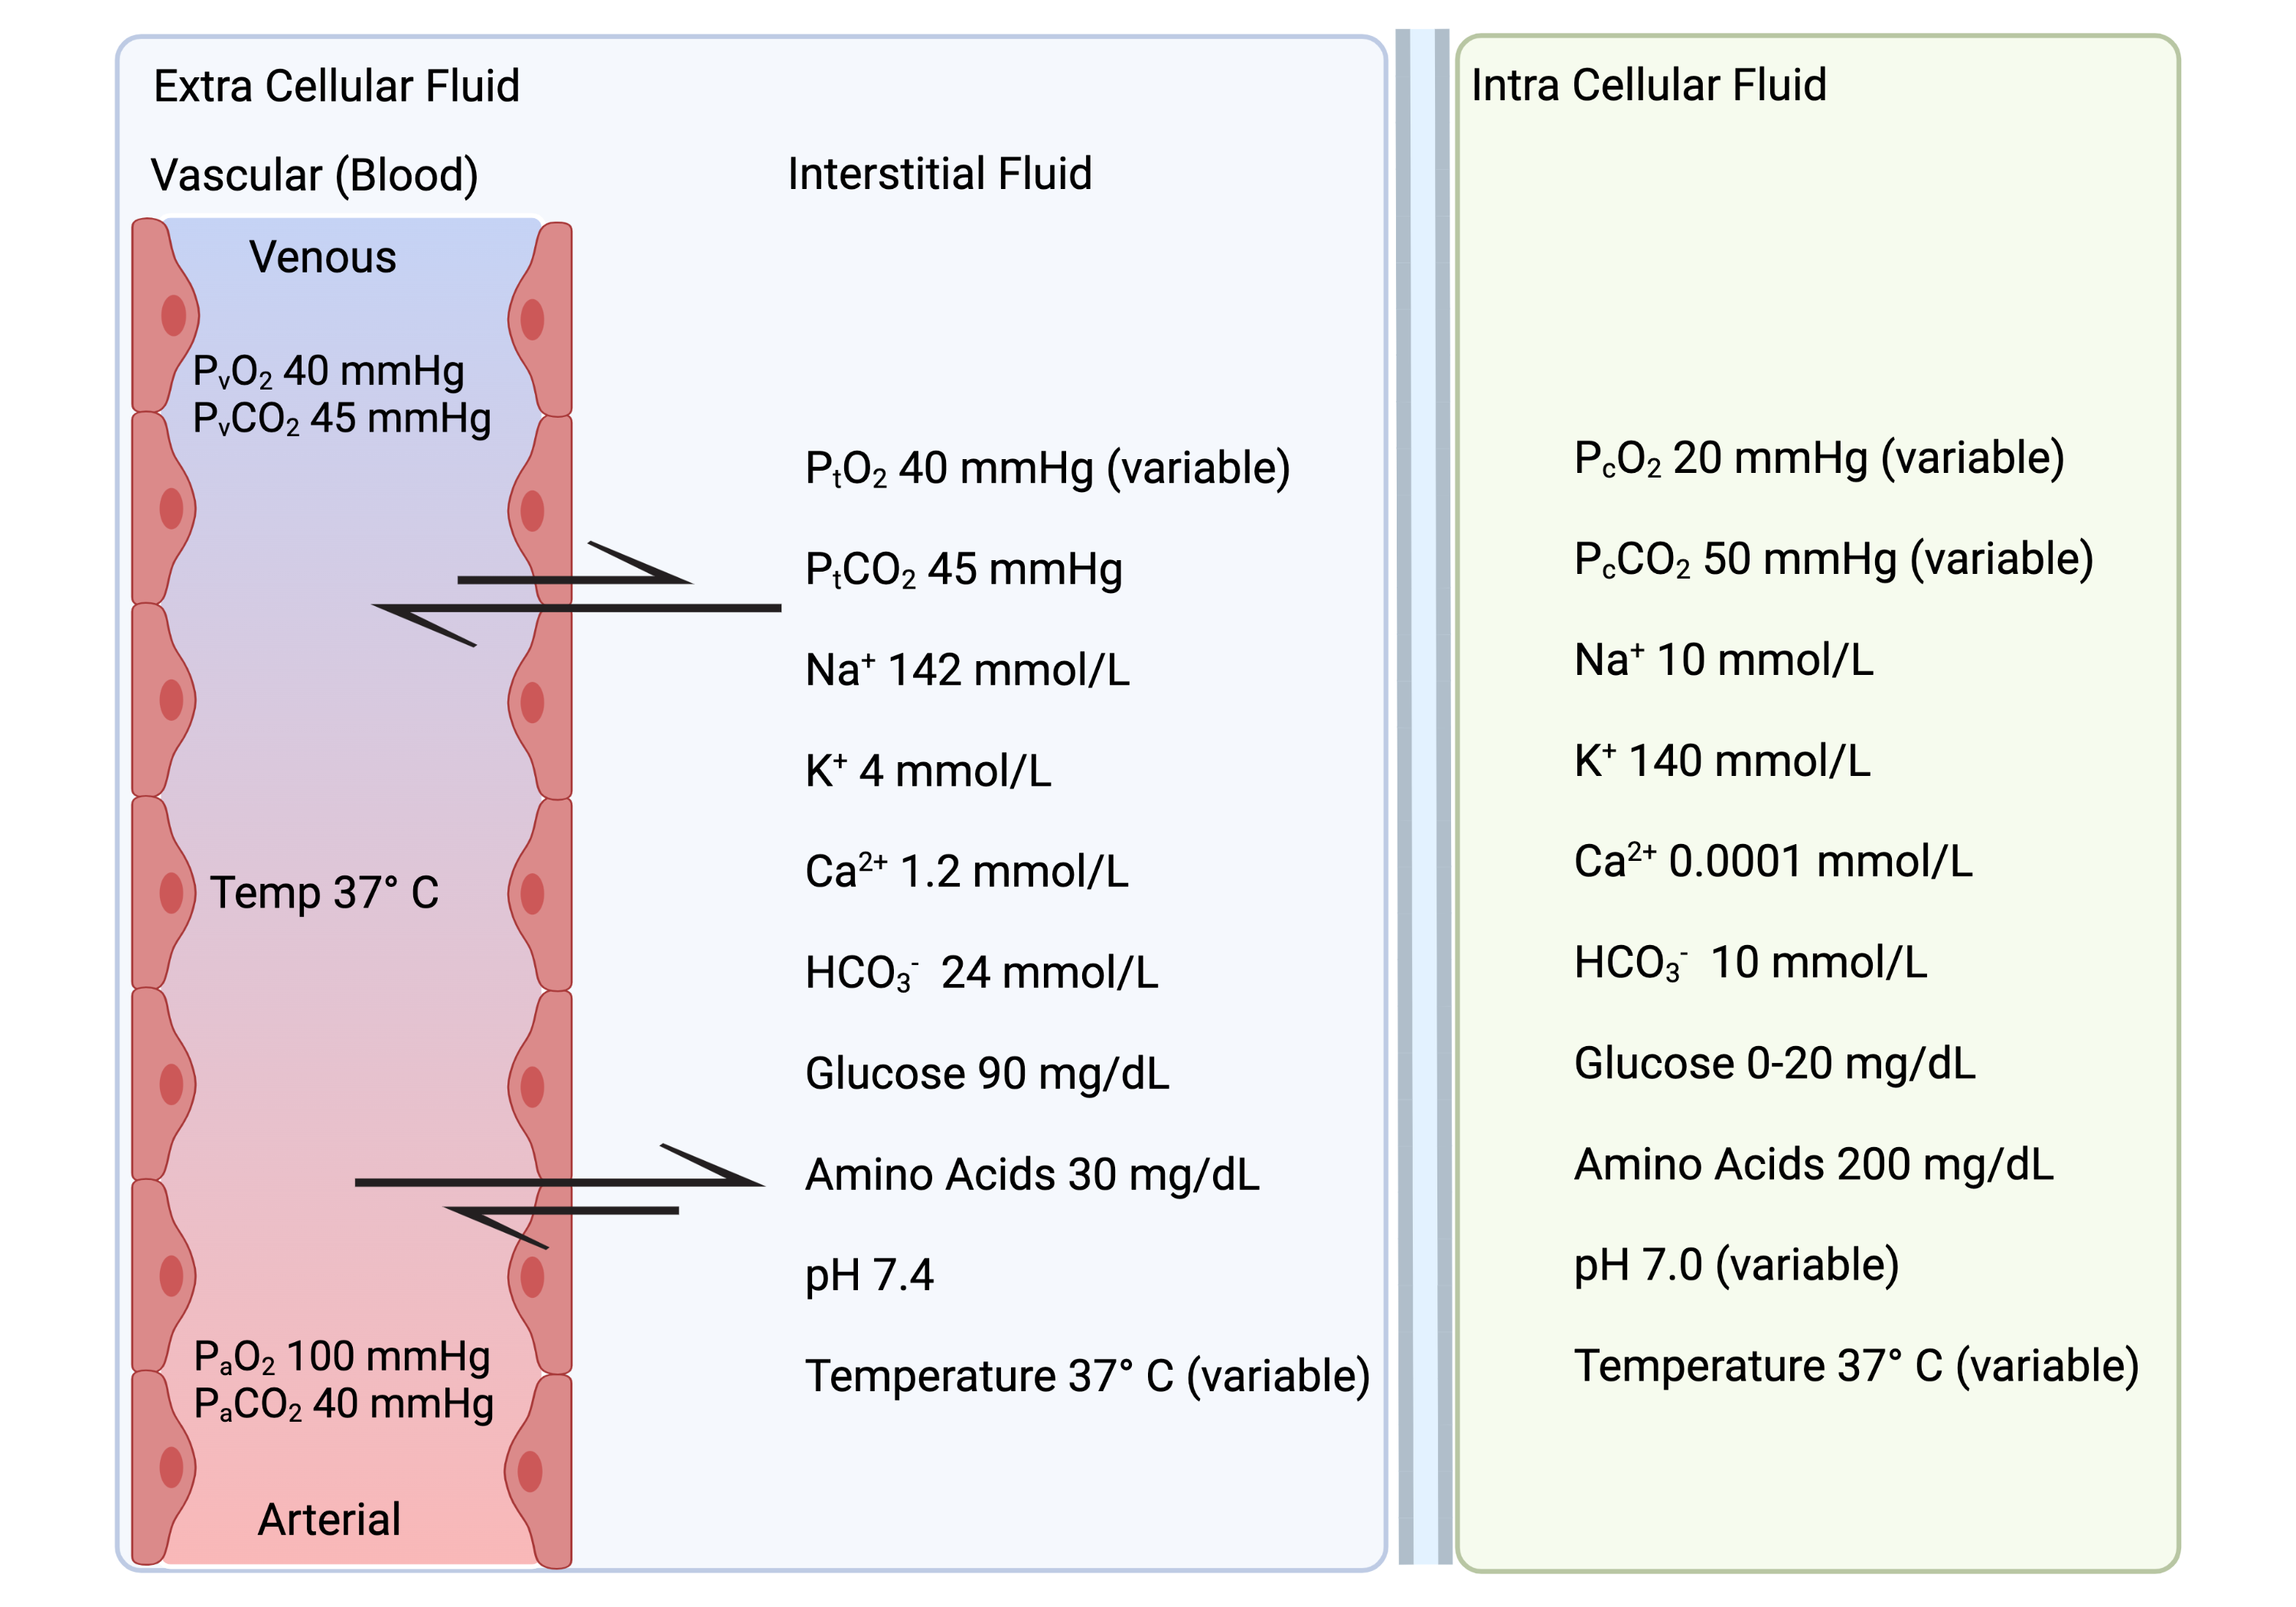
\includegraphics[width=1.0\linewidth]{./figure/ecf.png}
    \caption{Extra-cellular (Vascular \& Interstitial) and Intra-cellular Fluid \footnotesize{(Created with BioRender.com)}}
    \label{fig:ecf_respiration}
\end{figure}

The diffusion of $O_2$ into the tissue (interstitial space) reduces the partial pressure of $O_2$ in the blood. The $PO_2$ at the venous end of the capillary is the $P_vO_2$. An important concept is that the $P_vO_2$ from different areas of the body can be quite different. The regional $P_vO_2$ depends on the regional metabolism. While the $P_aO_2$ is the same throughout the arterial circulation, the $P_vO_2$ is different throughout the venous circulation, but continues to mix and become similar until the final mixing chambers of the right atrium and ventricles are reached. In other words, the $P_vO_2$ in the right ventricle represents a weighted mean from the entire body. And it is the $P_vO_2$ from the right ventricle that gets sent to the lungs, which means all of the alveoli receiving blood get blood with the same $PO_2$.

\paragraph{Carbon Dioxide}

Partial pressure driven diffusion of $CO_2$ follows the same reasoning as above but in the opposite direction. The $P_cCO_2$ is the highest partial pressure which drives diffusion of $CO_2$ out of the cell into the interstitial fluid. The $P_tCO_2$ is higher than the $Pa_CO_2$ in the arterial blood at the arterial end of the capillary, which drives $CO_2$ into the capillary. The $P_cCO_2$ is variable based on the rate of $CO_2$ produced during aerobic metabolism (TCA). The diffusion of $CO_2$ into the blood increases the $PCO_2$ in blood flowing through the capillary. At the venous end the $P_vCO_2$ equilibrates to whatever is in the tissue which is higher than the $P_aCO_2$. There tends be wider fluctuation in $P_aCO_2$ than in $P_aO_2$ due to the much lower atmospheric partial pressure of $CO_2$. For reasons that will be partially elucidated in this chapter and more fully explained in Chapter \ref{chp:alveolar_oxygen} on Ventilation, variation in ventilation (breathing rate and volume) can create large fluctuations in $P_aCO_2$ with relatively little change in $P_aO_2$. 

\subsection{Factors Influencing Diffusion}

The factors influencing diffusion are provided in the following equation:
\vspace{4 mm}
\begin{equation}
    \dot{D} = \frac{A}{T} \times d \times (P_1 - P_2)
    \label{diffusion}
\end{equation}
\vspace{4mm}

\begin{itemize}
    \item $\dot{D}$ is diffusion as a rate (amount of substances over time)
    \item A is the surface area that diffusion can occur
    \item T is the thickness of the membrane through which diffusion can occur
    \item d is a diffusion coefficient that is related to the solubility and molecular weight of the substance diffusing
    \item $P_1 - P_2$ is the partial pressure gradient
\end{itemize}

Equation \ref{diffusion} assumes that the membrane is permeable to the substance being diffused. Which means there are no membrane restrictions to diffusion other than the surface area or thickness in the equation. Since that is the situation for the diffusion of $O_2$ and $CO_2$ across the cell membrane, capillary membrane and alveolar-capillary membrane this assumption is appropriate for respiration.

\paragraph{Diffusion of $O_2$ and $CO_2$}

Since a nearly equal amount of $O_2$ and $CO_2$ is diffused across the cell, capillary and alveolar-capillary membrane during the microcirculation of blood the diffusion rates are, for all intents and purposes, equal under physiological conditions. They are always crossing the same membranes and therefore have the same $A$ and $T$. Since, as can be seen in Figure \ref{fig:ecf_respiration} the partial pressure gradients ($P_1 - P_2$) are not equal, the diffusion coefficient ($d$) must be (and indeed) is different between $O_2$ and $CO_2$. As can be deduced from Equation \ref{diffusion}, $CO_2$ has a higher $d$ due to a higher solubility.\footnotemark\footnotetext{This relationship between solubility, partial pressure and diffusion is much more complicated than this since not only does solubility influence the diffusion coefficient and the rate of diffusion for a given partial pressure gradient, but solubility is inversely proportional to the partial pressure of the substance that is soluble based on Henry's law. These factors are beyond the depth of this text \cite{christmas_equations_2017}.}



\section{Blood Transport}

Whether discussing venous blood (from tissues and cells to the lungs), or arterial blood (from the lungs to the tissues and cells), $O_2$ and $CO_2$ are being transported in the blood. The transport of $O_2$ and $CO_2$ in the blood has overlap (shared mechanisms) albeit with different proportions per mechanism. Overall, $CO_2$ has an additional transport option that is responsible for a large proportion of $CO_2$ transport.

A small amount of $O_2$ (approximately 1-2\%) and $CO_2$ (approximately 7\%) is transported simply as $O_2$ and $CO_2$ in the blood. This portion contributes to the partial pressures and therefore has a large role to play in diffusion and as a factor in determining the amount being carried in the blood. But it is clearly not the largest quantity of either $O_2$ or $CO_2$ being transported.

\subsection{Red Blood Cells}

Red blood cells (RBCs), also referred to as erythrocytes, constitute approximately 45\% of the total blood volume (Hematocrit, HcT). RBCs do not have a nucleus and therefore do not divide. They are regenerated and replaced regularly in the bone marrow through the process called erythropoiesis. Erythropoiesis is stimulated by the hormone erythropoietin (EPO) which is released from the kidneys.

%Add the life cycle of RBCs figure
\begin{figure}
    \centering
    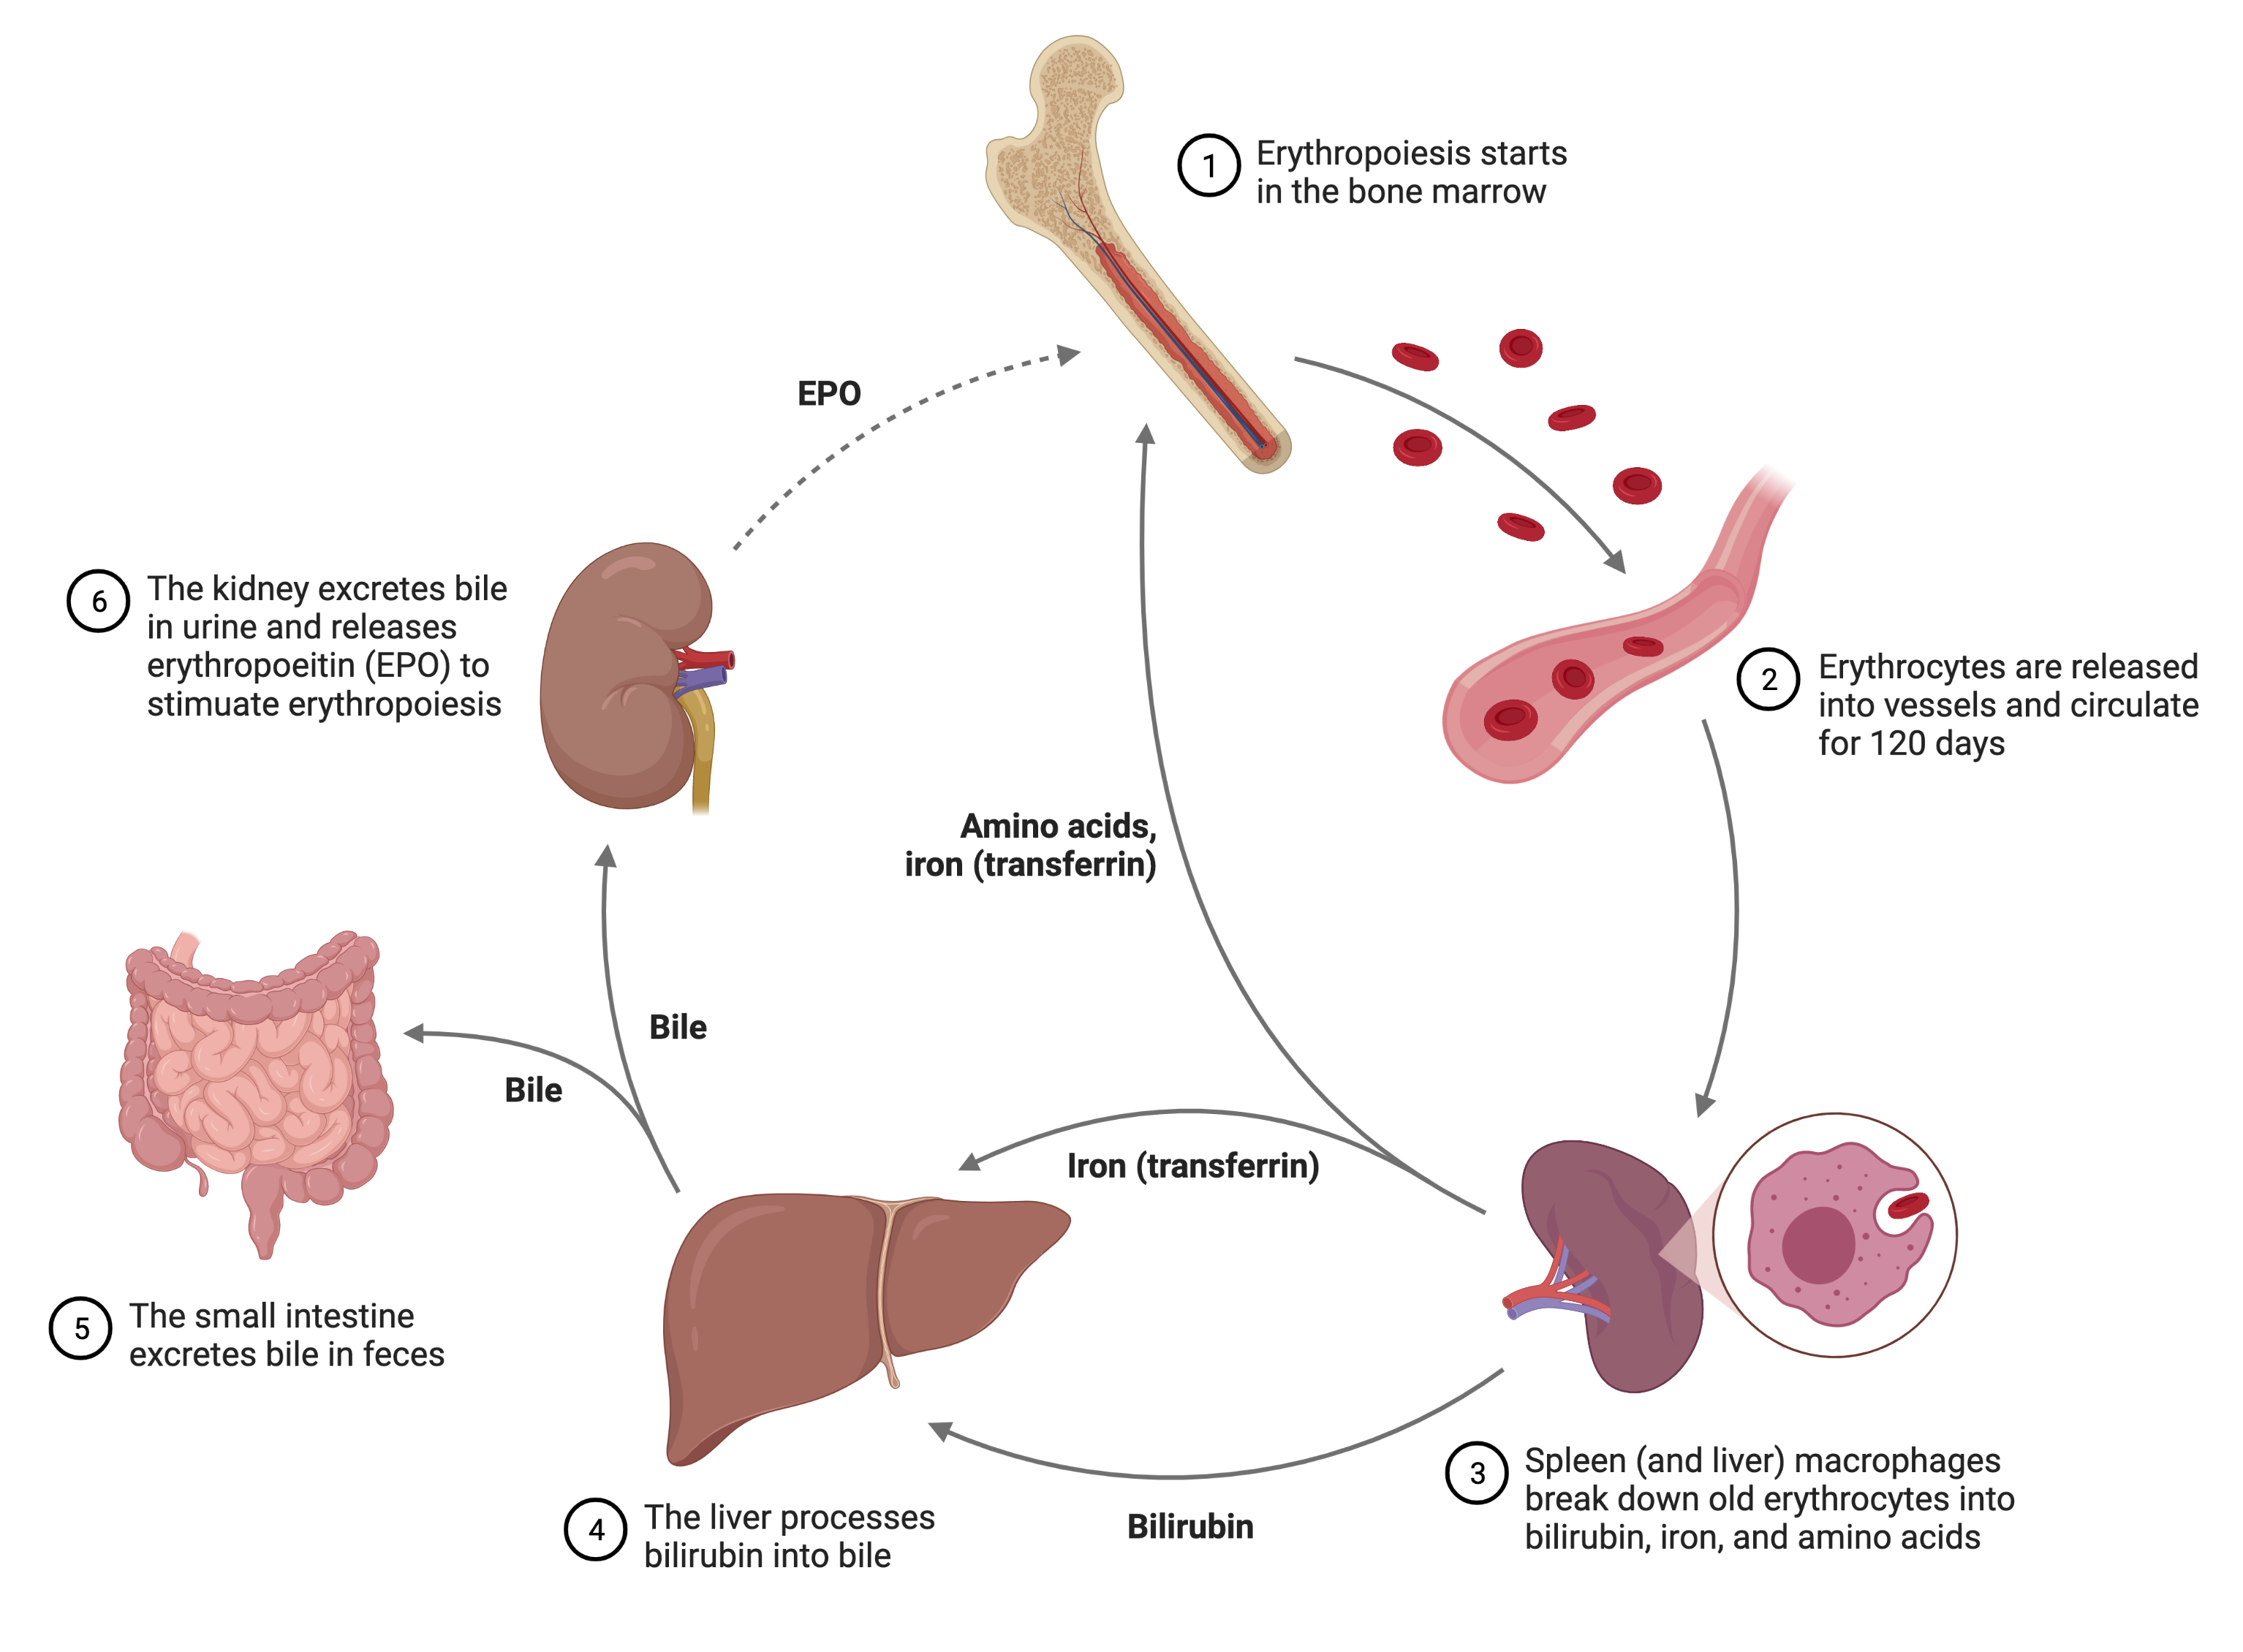
\includegraphics{./figure/RBC.png}
    \caption{Life Cycle of Erythrocytes \footnotesize{(Created with RioRender)}}
    \label{fig:RBC}
\end{figure}

EPO is secreted by the kidneys at a regular rate, possibly in response to bile filtration, to compensate for normal cellular turnover (See Figure \ref{fig:RBC}). EPO release increases in response to cellular hypoxia and stimulates additional erythropoiesis as a compensatory mechanism in an attempt to solve the problem of cellular hypoxia. Common causes of cellular hypoxia resulting in elevated levels of EPO include altitude or low barometric pressure (hypobaric) exposure which reduce environmental and therefore arterial $PO_2$; anemia (reduced RBCs), and hypoxemia due to chronic lung disease. RBCs contain hemoglobin (HgB). 

Hgb is the iron-containing oxygen-transport protein. While HcT is the percent of blood that is composed of RBCs, HgB is the number of grams per liter of HgB in blood (usually per deciliter or 100 milliliter\footnotemark\footnotetext{1 $dL$ is equal to 100 $mL$}). A normal HgB level is approximately 15 $g/dL$ with a range 12 to 20 $g/dL$.

HgB has an $O_2$-binding capacity of 1.34 $mL O_2 / g$ which increases the total blood oxygen capacity seventy-fold compared to dissolved oxygen in blood. A HgB molecule can carry up to four oxygen molecules. When fully saturated with $O_2$ and with a HgB of 15 $g/dL$, there is approximately ($15 \times 1.34 = 20.1 mL O_2/ 100 mL$ of blood. This estimate varies predictably and proportional to the amount of actual saturation and HgB.

%Anemia section
\paragraph{Anemia}
Anemia with HcT in the range of 0.3 - 0.4 is common following surgery and a cause of fatigue and reduced endurance that will recover in several days when kidneys are healthy due to an increase in EPO release and associated erythropoiesis (or sooner if facilitated by a blood, or RBC, transfusion). Causes of anemia that are not reversible, and that continue until anemia progresses until HcT is less than 0.1, can result in death. Anemia is a, but not the only, cause of hypoxemia. With anemia, there is reduced oxygen carrying capacity in the blood.

% Consider expanding anemia section

\paragraph{Transfusions \& ABO Blood Types}

RBCs can have antigens on their cell membrane that are named A and B. Blood can occur with three possible types, A, B, AB or O (O being an indication that the RBC membrane has neither A or B antigens. Whatever antigen an RBC membrane has, it's plasma contains anti-bodies for the opposite antigen. If A antigen is present on the RBC then the plasma has Anti-B antibodies. If A and B antigen is present (AB blood) then the plasma has neither antibody. If no antigen is present (O blood) then the plasma has both antibodies. The type of blood influences whether the blood can be donated or received as summarized in Figure \ref{fig:ABO}.

%Add ABO blood type figure

\begin{figure}
    \centering
    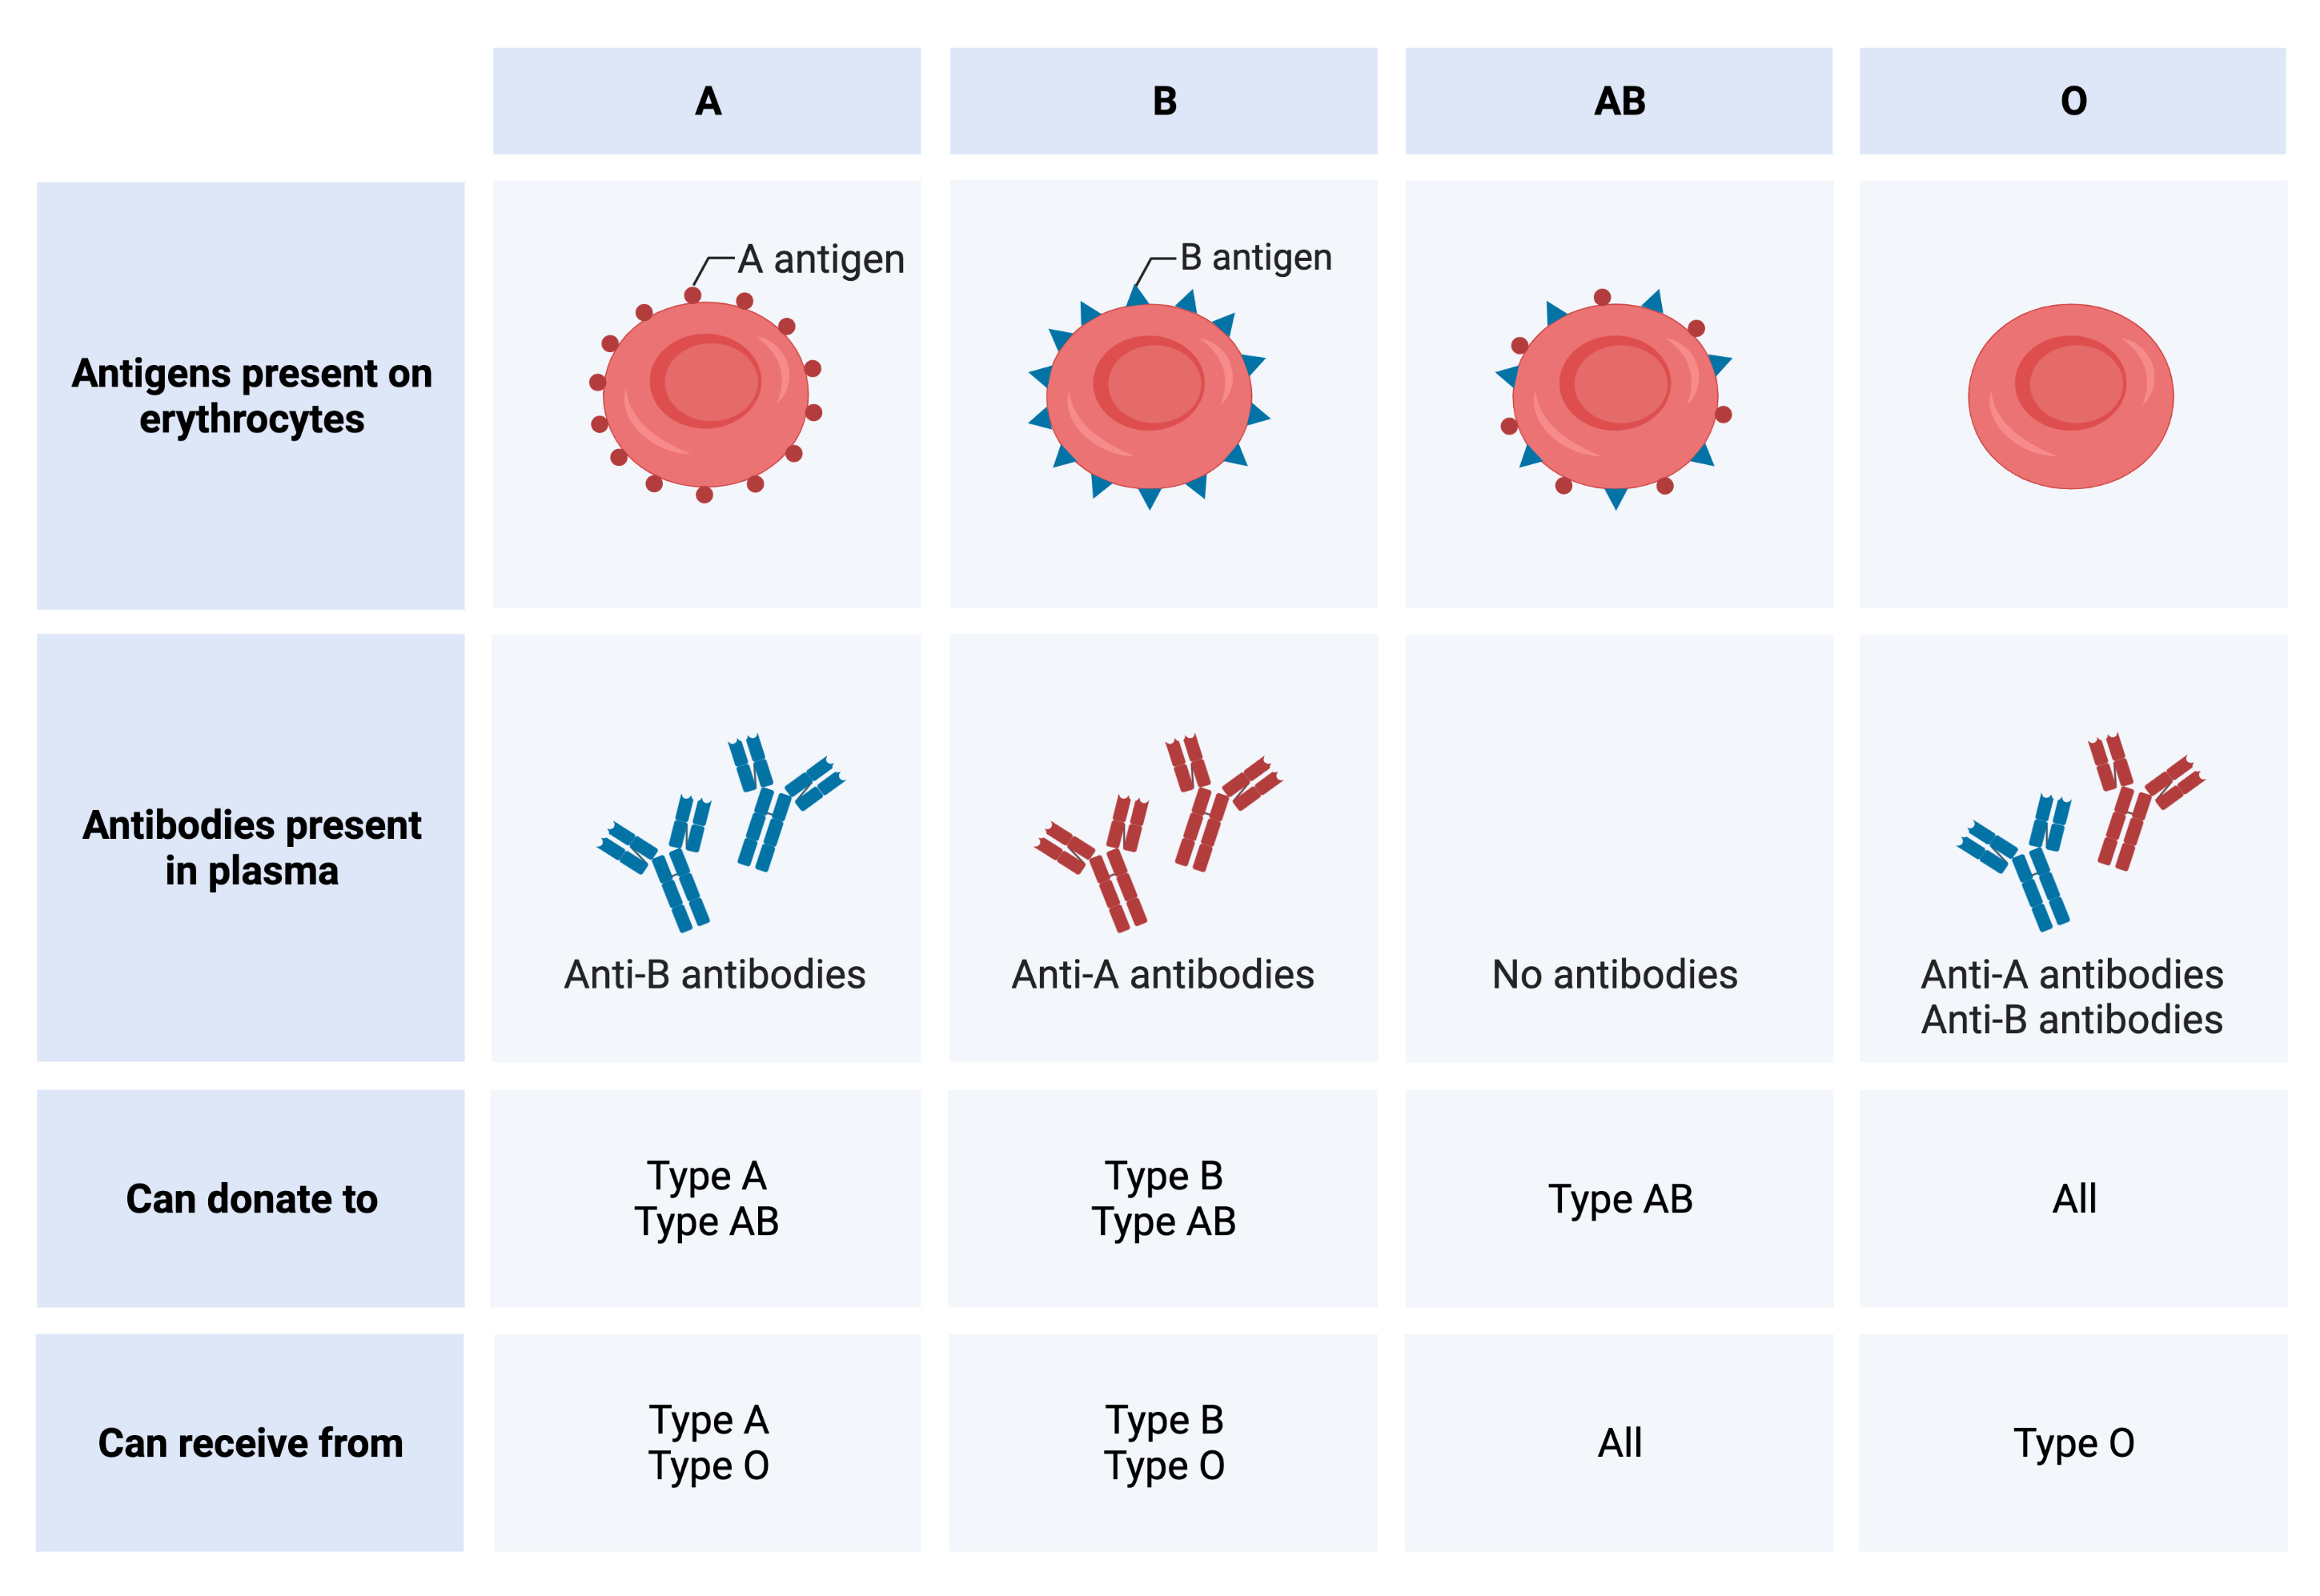
\includegraphics{./figure/ABO.png}
    \caption{ABO Blood Types}
    \label{fig:ABO}
\end{figure}

\subsubsection{Blood Transport of $CO_2$}

$CO_2$ is transported directly in the blood in a small quantity (7\%) which generates the partial pressure of $CO_2$ in the blood ($P_aCO_2$ in arterial blood, and $P_vCO_2$ in the venous blood). 

The majority of $CO_2$ is transported as bicarbonate ($HCO_3^-$) (approximately 70\%) through the following chemical reaction within the red blood cells (RBCs). 
Within the RBC $CO_2 + H_2O \rightarrow H_2CO_3$ which is facilitated by the enzyme carbonic anhydrase. To buffer this acid, a hemoglobin (HgB) will bind with $H^+$ to form $HgB-H^+$ (which stays in the RBC) and a molecule of $HCO_3^-$ which is released into the plasma through an exchange with $Cl^-$ in a process known as the chloride shift.

% Consider adding a figure such as page 33 in the ppt

The remaining $CO_2$ (approximately 23\%) binds directly with HgB to form $HgB-CO_2$ which is referred to as carbaminohemoglobin (not to be confused with carboxyhemoglobin which is $HgB-CO$ from the inhalation of carbon monoxide, the result being carbon monoxide poisoning). 

These processes are facilitated by the movement of $CO_2$ into the RBCs which occurs due to the $PCO_2$ gradient between the plasma and the RBC. As the above reactions proceed the RBC $PCO_2$ drops and $CO_2$ will diffuse into the RBCs until the $PCO_2$ in the plasma and the RBC are equalized. As a reminder, gradient that pushes $CO_2$ into the plasma and then the RBCs originates in the mitochondria where $CO_2$ is being generated.


\subsection{Blood Transport of $O_2$}

$O_2$ is transported directly in the blood in a small quantity (1-2\%) which generates the partial pressure of $O_2$ in the blood ($P_aO_2$ in arterial blood, and $P_vO_2$ in the venous blood). 

The majority of $O_2$ is transported in RBCs, attached to HgB. The partial pressure ($PO_2$) gradients facilitate the movement across membranes, including into the RBCs, which then allow $O_2$-HgB binding. The affinity for $O_2$-HgB binding is related to the $PO_2$ as well as to the number of binding sites of a HgB molecule already bound with $O_2$. With each binding site that has an $O_2$ bound to it, there is an increased affinity for the other binding sites to bind. The binding of $O_2$ to HgB is also influenced by the temperature (increased temperature reduces $O_2$-HgB affinity), and the pH (acidity reduces $O_2$-HgB affinity), as well as a 2,3-bisphosphoglycerate (BPG) (increased BPG reduces affinity). BPG is found in RBCs and preferentially binds to HgB when $O_2$ is not bound to HgB. However, if there is an increase in BPG there is reduced affinity of HgB to bind with $O_2$. At first this sounds negative. However, as we will discuss soon, reducing the affinity of HgB for $O_2$ is helpful when the goal is to release $O_2$ so that it can diffuse into the metabolically active cells requiring $O_2$.

The relationship between the $PO_2$ and the amount of $O_2$ bound to HgB expressed as the percentage of binding sites of HgB with $O_2$ (oxygen saturation, $SO_2$) is given in the oxyhemoglobin saturation curve. The features of this curve depict, first, the relationship between $PO_2$ and $SO_2$; and shifts in the curve depict the influence of pH, $PCO_2$, temperature, and BPG. The curve is usually considered from the perspective of arterial blood and therefore the relationship between $P_aO_2$ and $S_aO_2$. When considering $P_aO_2$ and $S_aO_2$ the oxygen content of arterial blood that is being delivered is being assessed, reduced values indicate hypoxemia. However it is equally valid to consider the curve in the capillary or venous blood when considering the utilization of $O_2$ by the cells of the body; and the influence of the $O_2$-HgB affinity on releasing $O_2$ into the tissues.
Note, when $S_aO_2$ is estimated with a pulsed oximeter it is abbreviated as $S_p_O_2$.

% Add some oxyhemoglobin dissociation curves and further discussion



\section{Pulmonary Circulation}

The majority of pulmonary circulation is to the alveoli (small air sacs of the lung). Alveolar circulation is a low pressure - high volume system with such a high density of capillaries that the blood flows almost as sheets in close contact surrounding the alveoli. Blood leaving the right ventricle (RV) flows into pulmonary arteries (venous blood) and into the alveolar circulation for respiration (gas exchange) with the alveoli to become arterial blood. After flowing through the capillaries of the alveoli this arterial blood returns to the left atrium (LA) through the pulmonary veins. 
Approximately 1-2\% of cardiac output is sent to the bronchial arteries of the lungs for oxygenation of lung cells. This circulation is from the systemic circulation (from the left ventricle), but it returns its venous blood to the heart through the pulmonary veins into the LA. This small amount of venous blood mixes with the otherwise arterial blood in the LA and has a minor, inconsequential, effect on the $P_aO_2$ and $S_aO_2$.

\paragraph{Pulmonary Circulation Pressures}

Pulmonary artery pressure (PAP) is synonymous with arterial blood pressure (BP) and has both systolic and diastolic components. PAP is much lower than BP under normal circumstances, approximately 15-30 $mmHg$ / 5-10 $mmHg$ with pulmonary capillary pressures approximately 7 $mmHg$. Central pulmonary venous pressure is the pressure in the LA, approximately 0-2 $mmHg$, which is similar to the central systemic venous pressure in the RA. 

Intensive (critical) care unit (ICU) monitoring for patients with cardiac or other blood flow or volume conditions are often monitored with a cathether that records pressure in the pulmonary artery for continuous PAP monitoring that can occasionally be pushed further into the pulmonary circulation to estimate the pulmonary capillary pressure with a measurement referred to as the pulmonary capillary wedge pressure (PCWP). The PAP and PCWP are utilized to assess whether left sided heart function is adequate for the current blood volume, or whether the pulmonary circulation pressures are rising. If the pulmonary circulation pressures are too high then the pulmonary microcirculation favors filtration which could result in pulmonary edema or effusion.

% Left off here

\paragraph{Pulmonary Microcirculation \& Lymphatics}



\section{External (Alveolar) Respiration}



\paragraph{Atmospheric Limits}

The atmospheric $PO_2$ places a limit on how high the alveolar partial pressure ($P_AO_2$) can be and therefore how high the $P_aO_2$ can be. This upper limit means now matter how much someone breathes, there is an upper limit on diffusion of oxygen into the blood. That upper limit is reduced with lower atmospheric $PO_2$.


\section{\textit{Connections:} Respiration Vital Signs}

\printbibliography[heading=subbibintoc]